\section{Binding Flaws in Audited Applications}\label{sec:study}

We ask how common binding flaws are, how severe, and which patterns dominate
(RQ1). Professional audits are the best available record: each finding was
found by an expert, argued in writing, and usually fixed.

\subsection{Collecting and labeling findings}\label{sec:study-collect}

\para{Sources and screening}
We enumerated 8,578 unique public audit reports from 68 sources: audit firms
with ZK practices (e.g., Veridise, Zellic, zkSecurity, Trail of Bits, ABDK,
OpenZeppelin, Consensys Diligence), contest platforms (Code4rena, Sherlock,
Cantina) and advisory databases. A report is in scope if it audits an
application that verifies a ZK proof and acts on it: 343 reports pass, 322
after deduplication by URL, of which 311 publish their finding text; 311 is
the denominator of every per-report rate below. From them we logged 698
findings that touch proof verification, public inputs, nullifiers, keys or
the use of verified values (662 unique), screened them to 300 candidates, and
labeled all of them except those triaged as likely not binding, plus a random
sample of 14 of those to check the triage: 264 items. As a completeness
check, the sweep recovered 49 of 50 binding findings in an independently
assembled list of known cases.

\para{Labeling}
Each candidate was labeled against a written guide that defines C1--C3, the
five patterns, the exclusions of Section~\ref{sec:definition} and worked
examples (Appendix~\ref{app:labels}). A label records binding (Y/N/U),
pattern, whether the issue is a proof-system soundness bug, C1--C3
individually, the effect, the unbound value, the intended policy $\Pi$ and
confidence. Labels were proposed by an LLM and adjudicated by two raters who
discussed every item. For the 51 items with a public repository and
vulnerable commit they recorded $\Pi$ from the code and documentation, and
every item used in the tool evaluation received a second, code-level pass
that located the flaw in the source. \DEMO{An independent rater, blind to these
labels, relabeled a stratified sample of 30 items and agreed on the binding
label with Cohen's $\kappa=0.78$ and on the pattern with $\kappa=0.71$.
Re-applying the policy rule to all binding labels changed two of them in
opposite directions, leaving the counts unchanged.} Removing 4 duplicates and
5 undecidable items leaves 255 findings.

\subsection{Prevalence, severity and patterns}\label{sec:study-prev}

\begin{table*}[t]
\centering
\caption{Representative auditor-reported binding flaws (public reports; all
fixed or acknowledged). Severity is the auditor's.}
\label{tab:examples}
\footnotesize
\begin{tabular}{@{}llllp{4.3cm}p{4.6cm}@{}}
\toprule
\textbf{Pattern} & \textbf{Project} & \textbf{Auditor} & \textbf{Sev.} & \textbf{Effect} & \textbf{Unbound value} \\
\midrule
P1 & Nocturne & Zellic & Low & pays the reserved gas refund & refund recipient = \texttt{msg.sender} of the bundle \\
P1 & Taiko / Surge & Nethermind & High & records the bond receiver of a proven batch & bond receiver = \texttt{msg.sender} of the prover call \\
P1 & Arianee & Veridise & Critical & spends an issuer credit via a nullifier & the action the credit pays for \\
P2 & MorphL2 & Sherlock & High & resolves a state challenge & previous state root of the batch \\
P2 & vlayer & Veridise & Critical & acts on a proven contract-call result & chain ID of the proven execution \\
P2 & MACI & HashCloak & Critical & stores the new tally commitment & starting tally of the first batch \\
P3 & Anon Aadhaar & PSE & High & marks a vote nullifier used & nullifier derived from the photo only \\
P3 & ZkDrops & K.\ Gurkan & -- & transfers an airdrop, marks nullifier & raw 256-bit nullifier ($x$ and $x{+}r$ both verify) \\
P4 & Taiko / Surge & OpenZeppelin & Critical & accepts a proof for a batch of L2 blocks & guest program ID not pinned \\
P5 & Anon Aadhaar & PSE & Critical & acts on revealed identity attributes & which attribute sits at which index \\
\bottomrule
\end{tabular}
% src: dataset/labels-v1/LABELS-v1.csv (FULL, binding Y): L015, L041, L043, L014, L050, L048, L020, L049, L019, L007
\end{table*}


87 of the 255 findings (34\%) are core binding flaws; with 16 adjacent
proof-system soundness findings the total is 103 (40\%). The core findings
occur in 43 of the 68 project families, so they are not concentrated in a few
careless codebases. For contrast, 48 non-binding findings are
circuit-internal under-constraints that do not change what the consumer is
told, the class existing ZK tools target.

\begin{figure*}[t]
\centering
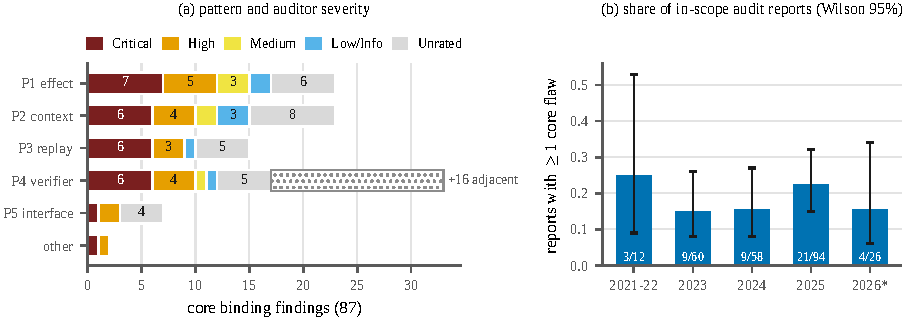
\includegraphics[width=\textwidth]{fig-study.pdf}
\caption{The 87 core binding findings. (a) Pattern by auditor severity; the
hatched bar adds the 16 adjacent proof-system findings that we exclude from
the core class. (b) Share of in-scope ZK application audit reports with at
least one core finding, by report year (2026 partial; 61 undated reports
omitted). The 2023--2025 trend is not significant (Cochran--Armitage
$p=0.22$).}
\label{fig:study}
\end{figure*}

Figure~\ref{fig:study}(a) breaks the core findings down by pattern and
auditor severity. 46 of the 87 are rated Critical or High, which is 78\% of
the 59 with a rating (81\% with the adjacent findings); only 7 are Low or
Informational. Unrated findings are mostly contest and advisory entries
without a severity scale. Unbound effects (P1, 23) and missing context (P2,
23) dominate, followed by replay and aliasing (P3, 15) and verifier
integration (P4, 17). Interface mismatches (P5, 7) are rare, plausibly
because a mismatch usually makes honest proofs fail, which tests notice. The
unbound value varies widely---a refund address, a bond receiver, a prior
state root, a chain ID, a zkVM program ID, the position of an attribute in
the public-input array (Table~\ref{tab:examples})---but
the failure is always the same: the consumer acts on something the
statement does not fix.

\finding{Binding flaws are a major and severe class: 87 auditor-reported core
instances in 43 of 68 project families, 78\% of the rated ones Critical or
High. Unbound effects and missing context, the ZK analogues of signing too
little, account for over half.}

\subsection{Rate, auditors, layers and fixes}\label{sec:study-trend}

\para{Rate}
Raw counts grow (11 core findings in 2023, 19 in 2024, 32 in 2025), but so
does the number of ZK audits. Normalized, the share of in-scope reports with
at least one core finding is 0.15 in 2023, 0.16 in 2024 and 0.22 in 2025
(Figure~\ref{fig:study}b); the change is not significant ($p=0.22$; $p=0.12$
with adjacent findings), so we claim no rising rate. Over all 311 reports, 55
(18\%) report at least one core binding flaw: about one ZK application audit
in six.

\para{Auditors}
The 87 core findings come from 21 auditors and advisory sources, and no
single source contributes more than 21. Binding is a class that many
experienced auditors encounter, not the checklist item of one firm.

\para{Layers}
\DEMO{We tagged each core finding with the code a reviewer must read to decide
it, treating the statement side as known when the report states what the
proof establishes. Under this rule, 49\% can be decided from the consumer
alone, 23\% from the circuit or guest alone and 8\% only by comparing the
two; 20\% lie in verifier, recursion or framework code. The rule favors
single-layer tags, because the auditor has already done the cross-layer
reading and written it down: if a finding counts as cross-layer whenever its
fix adds a value to the statement, the consumer-only share falls to 32\%.
Even consumer-only findings require knowing \emph{which values the statement
fixes}, which no contract analyzer models.}

\para{Fixes}
\DEMO{Fixes mirror signature-misuse remedies. 56\% (49 of 87) add the missing
value to the statement, bind a context or make the replay key unique; 34\%
pin the verifier or program, check its result, or enforce a canonical
encoding. Only 6 findings were fixed by constraining a value the circuit
already exposed, the remedy a circuit analyzer would suggest.}

\finding{About one ZK application audit in six reports a core binding flaw.
Deciding one requires knowing what the statement fixes, wherever the flaw
sits; Section~\ref{sec:design} automates that reasoning.}
